%===========================================================
% This is the thesis template for the Statistics major at
% Amherst College. Brittney E. Bailey (bebailey@amherst.edu)
% adapted this template from the Reed College LaTeX thesis
% template in January 2019 with major updates in April 2020.
% Please send any comments/suggestions: bebailey@amherst.edu

% Most of the work for the original document class was done
% by Sam Noble (SN), as well as this template. Later comments
% etc. by Ben Salzberg (BTS). Additional restructuring and
% APA support by Jess Youngberg (JY). Email: cus@reed.edu
%===========================================================

\documentclass[12pt, twoside]{amherstthesis}
\usepackage{graphicx,latexsym}
\usepackage{amsmath}
\usepackage{amssymb,amsthm}
\usepackage{longtable,booktabs} %setspace loaded in .cls
\usepackage[hyphens]{url}
\usepackage{hyperref}
\usepackage{lmodern}
\usepackage{float}
\floatplacement{figure}{H}
\usepackage{rotating}
\usepackage{fancyvrb}
% User-added packages:
% End user-added packages

%===========================================================
% BIBLIOGRAPHY FORMATTING

% Next line commented out by CII
%%% \usepackage{natbib}
% Comment out the natbib line above and uncomment the
% following two lines to use the new biblatex-chicago style,
% for Chicago A. Also make some changes at the end where the
% bibliography is included.
%\usepackage{biblatex-chicago}
%\bibliography{thesis}


%===========================================================
% HYPERLINK FORMATTING

% Added by CII (Thanks, Hadley!)
% Use ref for internal links
\renewcommand{\hyperref}[2][???]{\autoref{#1}}
\def\chapterautorefname{Chapter}
\def\sectionautorefname{Section}
\def\subsectionautorefname{Subsection}
% End of CII addition
\usepackage{xcolor}
\hypersetup{
    colorlinks,
    linkcolor={red!50!black},
    citecolor={blue!50!black},
    urlcolor={blue!80!black}
}

%===========================================================
% CAPTION FORMATTING

% Added by CII
\usepackage{caption}
\captionsetup{width=5in}
% End of CII addition

%===========================================================
% TITLE FORMATTING

\renewcommand{\contentsname}{Table of Contents}

\usepackage{titlesec}
%%%%%%%%
% How to use titlesec:
% \titleformat{⟨command⟩}[⟨shape⟩]{⟨format⟩}{⟨label⟩}{⟨sep⟩}
%  {⟨before-code⟩}[⟨after-code⟩]
%%%%%%%%

\titleformat{\chapter}[hang]
{\normalfont%
    \Large% %change this size to your needs for the first line
    \bfseries}{\chaptertitlename\ \thechapter}{1em}{%
      %change this size to your needs for the second line
    }[]

\titleformat{\section}[hang]
{\normalfont%
    \large % %change this size to your needs for the first line
    \bfseries}{\thesection}{1em}{%
     %change this size to your needs for the second line
    }[]

\titleformat{\subsection}[hang]
{\normalfont%
    \normalsize % %change this size to your needs for the first line
    \bfseries}{\thesubsection}{1em}{%
     %change this size to your needs for the second line
    }[]

% \titleformat{\section}[display]
% {\normalfont%
%     \large% %change this size to your needs for the first line
%     \bfseries}{\chaptertitlename\ \thechapter}{20pt}{%
%     \normalsize %change this size to your needs for the second line
%     }


%===========================================================
% DOCUMENT FONT

% \usepackage{times}
% other fonts available eg: times, bookman, charter, palatino


%===========================================================
% PASSING FORMATS FROM RMD --> LATEX

%%%%%%%%
% NOTE: Dollar signs pass parameters between YAML inputs
% in index.Rmd and LaTeX
%%%%%%%%

\Abstract{
The abstract should be a short summary of your thesis work. A paragraph is usually sufficient here.
}

\Acknowledgments{
Use this space to thank those who have helped you in the thesis process (professors, staff, friends, family, etc.). If you had special funding to conduct your thesis work, that should be acknowledged here as well.
}

\Dedication{

}

\Preface{

}

% Formatting R code display
% Syntax highlighting #22

% Formatting R code: set baselinestretch = 1.5 for double-spacing
\DefineVerbatimEnvironment{Highlighting}{Verbatim}{
  baselinestretch = 1,
  commandchars=\\\{\}}

% Formatting R output display: set baselinestretch = 1.5 for double-spacing
\DefineVerbatimEnvironment{verbatim}{Verbatim}{
  baselinestretch = 1,
  % indent from left margin
  xleftmargin = 1mm,
  % vertical grey bar on left side of R output
  frame = leftline,
  framesep = 0pt,
  framerule = 1.5mm, rulecolor = \color{black!15}
  }

\title{My amazing title}
\author{Tony Ni}
\date{April DD, 20YY}
\division{}
\advisor{Brittney Bailey}
% for second advisor
\institution{Amherst College}
\degree{Bachelor of Arts}
\department{Mathematics and Statistics}

% Fix from pandoc about cslreferences?
% https://github.com/mpark/wg21/issues/54
\newlength{\cslhangindent}
\setlength{\cslhangindent}{1.5em}
\newenvironment{cslreferences}%
  {\setlength{\parindent}{0pt}%
  \everypar{\setlength{\hangindent}{\cslhangindent}}\ignorespaces}%
  {\par}

% Added by CII
%%% Copied from knitr
%% maxwidth is the original width if it's less than linewidth
%% otherwise use linewidth (to make sure the graphics do not exceed the margin)
\makeatletter
\def\maxwidth{ %
  \ifdim\Gin@nat@width>\linewidth
    \linewidth
  \else
    \Gin@nat@width
  \fi
}
\makeatother

% ===========================================
% DOCUMENT SPACING

\setlength{\parskip}{0pt}
% Added by CII

\providecommand{\tightlist}{%
  \setlength{\itemsep}{0pt}\setlength{\parskip}{0pt}}


% ===========================================
% ===========================================
% ===========================================
\begin{document}

\doublespace
% Everything below added by CII
  \maketitle

\frontmatter % this stuff will be roman-numbered
\pagenumbering{roman}
\pagestyle{fancyplain}
%\pagestyle{fancy} % this removes page numbers from the frontmatter

  \begin{abstract}
    The abstract should be a short summary of your thesis work. A paragraph is usually sufficient here.
  \end{abstract}
  \begin{acknowledgments}
    Use this space to thank those who have helped you in the thesis process (professors, staff, friends, family, etc.). If you had special funding to conduct your thesis work, that should be acknowledged here as well.
  \end{acknowledgments}

  \hypersetup{linkcolor=black}
  \setcounter{tocdepth}{2}
  \tableofcontents

  \addcontentsline{toc}{chapter}{List of Tables}\listoftables

  \addcontentsline{toc}{chapter}{List of Figures}\listoffigures


\mainmatter % here the regular arabic numbering starts
\pagenumbering{arabic}
\pagestyle{fancyplain} % turns page numbering back on

\hypertarget{intro}{%
\chapter{Introduction}\label{intro}}

\hypertarget{background}{%
\section{Background}\label{background}}

Coal is one of the most dangerous combustible fuels which is being burned in all across the world as one of the largest methods of obtaining energy. Yet, although it is a fossil fuel which is naturally abundant and easy to utilize, it is comprised of a long list of dangerous chemicals including -- but not limited to: arsenic, radium, boron, and a large list of other chemicals which prove to be dangerous to humans and animals alike. (Kelderman et al., 2019)

Power plants produce electricity by burning this coal, and as a result of how prevalent it is within the US - over 100 million tons of coal ash are produced every year. This side-product as a result of the coal combustion is often disposed by directly being dumped into landfills and waste ponds. (Kelderman et al., 2019)

Only recently have these complaints and lawsuits regarding the disposing practices made by non-profit environmental organizations been heard. Due to the onslaught of pressure put on the Environmental Protection Agency -- the Coal Ash Rule was bor in 2015. (Kelderman et al., 2019)

This rule has forced over 265 coal power plants -- about 3/4 of all coal power plants in the US - to make data regarding chemical concentrations publicly available to the general population. (Kelderman et al., 2019)

In their analysis using this data, the Environmental Integrity Project -- a non-profit organization dedicated to issues involving environmental justice have concluded that essentially all groundwater under coal plants are contaminated. (Kelderman et al., 2019)

However, is this really the case? There are many naturally occurring chemicals existing in groundwater as as such, perhaps their claims are overstated.
\begin{figure}

{\centering 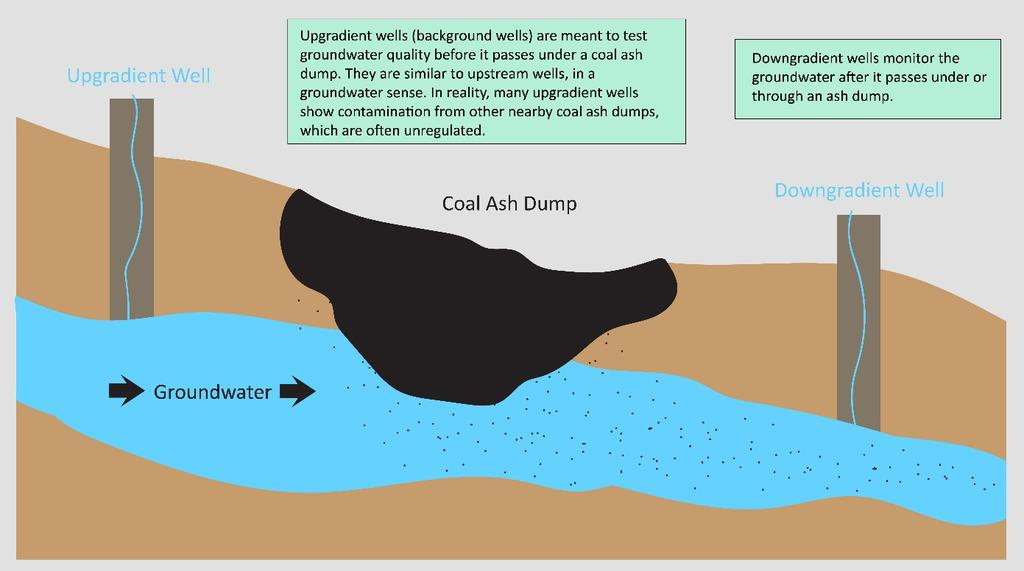
\includegraphics[width=1\linewidth]{figures/upgradientdowngradient} 

}

\caption{Difference Between Upgradient and Downgradient Wells}\label{fig:upgradientdowngradient}
\end{figure}
Typically in a coal ash plant, there exists two types of wells: upgradient wells and downgradient wells. These wells are essential to measure the amount of contamination being caused by coal ash. Upgradient wells, also known as background wells, measures the concentrations of chemicals in groundwater before it passes through an coal ash dump. Conversely, downgradient wells measure the concentrations of chemicals in groundwater after it passes through a coal ash dump.
\begin{itemize}
\tightlist
\item
  ``80\% of the US population is served by 14\% of the utilities,'' so if something were to get into the water distribution system, it can easily spread amongst the US population which is why contamination in water services is so important. (Byer \& Carlson, 2019)
\end{itemize}
With this information, typically -- one estimates the amount of chemical contamination caused by a coal as dump by subtracting the upgradient concentration from the downgradient concentration of a chemical (downgradient concentration - upgradient concentration).

However, due to the lack of proper reporting guidelines prior to the enactment of the Coal Ash Rule, we believe that there may be retired or even unregulated upgradient wells which can cause the concentrations of chemicals being recorded from these upgradient wells to be inaccurate or even completely wrong.

Our end goal remains the same as the EIP: to identify contaminated groundwater in coal plants -- but to attempt to find a way to effectively correct the improper/inaccurate values resulting from LOD errors and other factors which the EIP may not have considered.

The limit of detection problem stems from the measuring devices' inability to obtain chemical concentrations smaller than a certain threshold amount, thus affecting the measurements recorded.

Our plan is to utilize bootstrapping and imputation techniques to correct for these measurements by accounting for the innate contamination which may be caused by factors such as retired and unregulated wells that were mentioned before.

\hypertarget{data}{%
\section{Data}\label{data}}

\hypertarget{coalashrule}{%
\subsection{Coal Ash Rule}\label{coalashrule}}

A large coal ash spill at the Tennessee Valley Authority (TVA) which occured on December 22, 2008 in Kingston, TN -- prompted the Environmental Protection Agency (EPA) to propose a set of standardized regulations and procedures to address the concerns regarding coal ash plants nationwide in the US. (Environmental Protection Agency, 2020)

This was known as the Coal Ash Rule, passed on December 19, 2014. (Environmental Protection Agency, 2020)

Changes were made to the Coal Ash Rule over the years in the form of `amendments,' one of which made required facility information and data to be made publicaly available to the public (April 15, 2015 rule change) (Environmental Protection Agency, 2020)

\hypertarget{source-of-data}{%
\subsection{Source of Data}\label{source-of-data}}

The data used in the study are from the results published in ``Annual Groundwater Monitoring and Corrective Action Reports'' which were made available to the public in March 2018 as a result of the Coal Ash Rule. (Environmental Integrity Project, 2020)

These reports are in PDF format and are thousands of pages long, which makes it difficult for individuals to look through the data in a meaningful way. (Environmental Integrity Project, 2020)

The EIP obtained the data from an online, publicly available database containing groundwater monitoring results from the first ``Annual Groundwater Monitoring and Corrective Action Reports'' in 2018 which was collected from coal plants and coal ash dumps under the Coal Ash Rule (Environmental Integrity Project, 2020)

They wrangled the data into a more accessible machine-readable format which contains information from over 443 annual groundwater monitoring reports posted by 265 coal ash plants, which is downloadable from the EIP's website. (Environmental Integrity Project, 2020)

\newpage

\hypertarget{variables}{%
\subsection{Variables}\label{variables}}

The dataset contains information regarding chemical concentrations at coal plants. A coal plant consists of multiple disposal areas for the coal ash that it produces. At each disposal area, there are specific locations that groundwater is being measured, known as wells which represent an observation in the dataset. There are two types of wells -- upgradient and downgradient wells. The variables consist of information regarding the specific chemical concentrations of each well. From the 19 different contaminants (antimony, arsenic, boron, etc.) a major problem is that some wells only have measurements for certain chemicals and don't have them for others.

\hypertarget{plan-of-action}{%
\subsection{Plan of Action}\label{plan-of-action}}

Within the report, the EIP mentions certain restrictions within the data that have caused their data to potentially be inaccurate (specifically, with limit of detection problems, and a large amount of missing chemical data). The limit of detection problem comes when measuring devices used to measure chemical concentrations are unable to detect below a certain threshold, causing large numbers of observations to have duplicate, wrong values -- which can cause for misguided analysis.The other issue is less guided/formed, but for brevity, we think that a lot of the issues in the data comes from the potential possibility of contamination during data collection from investigators from non coal-ash sources. This may include things like: retired/unregulated wells which are old and have chemicals leaking into the groundwater, mismanagement in measuring, etc.My project hopes to work with methods on handling this missing data -- alongside investing potential uses of bootstrapping and other resampling methods (potentially?) in order to try to come up with a more statistically accurate and sound result by looking to assuage the problems that the EIP faced in their analysis. Specifically, to find a way to split up the data into ''uncontaminated'' and ''contaminated'' wells in order to find the natural distribution of chemicals in each -- and doing to so in the face of data corrupted by LOD problems and inaccuracies. I'm hoping to apply and compare different ways of altering the data to account for these myriad of issues in order to look for more salient findings that the EIP might have missed or if not, to see if improvements can be made regarding the way that contaminated coal ash wells are being identified.

\hypertarget{methodology}{%
\chapter{Methodology}\label{methodology}}

\hypertarget{overview}{%
\section{Overview}\label{overview}}
\begin{itemize}
\item
  The idea of missingness and incompleteness is commonplace throughout our world, and is even more prevalent within the statistical world. Known more formally as censoring, this condition exists when we have incomplete information regarding the values of a measurement within a dataset.
\item
  A specific instance of censoring which scientists crossing beyond fields exists in the form of left-censored data.
\item
  To understand this phenomena better, consider the following example. Imagine a scenario in which you are attempting to estimate the time at which the sun rises each morning. You wake up every morning far before the sun rises, at 3 A.M. and make sure to stay outside to witness the specific time at which you are able to see the sunrise, recording that time. However, on the first day of the study, you oversleep and wake up at 7:00 AM, with the sun already out. We now have an instance of left-censored data. We want to know the time at which the sun rose, but all we have is an upper limit value. All we know is that by 7:00 AM, the sun had already rose. The time at which the sunrise occurred could be any time before 7:00 AM, we have no knowledge on when that time could be.
\item
  As the scenario demonstrates, this form of censoring can often prove to be a thorn in the side, as the lack of certainty that we have in a measurement, often adds a layer of complexity within an analysis.
\item
  Left-censored values are also commonly referred to as limit of detection values, which will be used throughout this discussion.
\item
  What is the of detection (LOD)? LOD is often thought of as being closely related to analytical chemistry, but it lies close to the realm of statistics as well. By definition, a limit of detection is the lowest value reported which is different than the blank (generally zero) with some confidence level.
\item
  What is the problem with LOD? As a concept closely related to missing data, LOD values are often can lead to bad practices (in terms of statistical analysis) leading to analysis and/or conclusions which are heavily flawed as a result of someone misguided practices being used in the current statistical world in order to account for them.
\item
  An common malpractice used in order to account for left-censored practice is omitting these left-censored values from the analysis, which is of course the easiest way to deal with them -- but this approach discards a myriad of useful information (Berthouex, 2020)
\item
  These LOD entries still contain information that a lot of people don't realize -- specifically information that the values is between 0 and the LOD, which is actually very useful information. (Chen et al., 2011)
\item
  On the same vein, reporting limits can often be used be misleading as non-statisticians (practices in environmental law) may often interpret ND (non-detect) as nullity, when in fact it only means that the measurement falls below a certain limit (Elias \& Goodman, 1999)
\item
  Statisticians over past century have come up with methods to deal with this issue (some good\ldots{} and some\ldots{} kind of absolutely terrible). There are many different ways that researchers are dealing with detection limits, which are ubiquitous in the scientific realm. Some of the most common methods involve substitution, nonparametric, and maximum likelihood methods. (Lafleur et al., 2011)
\item
  Of course, these methods aren't the only way to deal with it, but it is what we have come up with for now. Detection limits are constantly changing as time passes and because of that -- techniques and ways to combat it will gradually evolve and change (for the better) to deal with it
\item
  Detection limits are constantly changing: as technology improves, so too does our ability to accurately measure substances (Elias \& Goodman, 1999)
\end{itemize}
\hypertarget{reporting}{%
\section{Reporting}\label{reporting}}
\begin{itemize}
\tightlist
\item
  The way that chemists/researchers indicate whether or not if a value is a LOD value or not varies across labs and as such isn't standardized\ldots{} Some may explicitly record \texttt{ND}, \texttt{\textless{}\ value} to indicate that an observation's value is left-censored. Others may simply record the value between 0 and LOD and not mark it as being left-censored at all (Berthouex, 2020)
\end{itemize}
\hypertarget{Approaches}{%
\section{Approaches}\label{Approaches}}
\begin{itemize}
\item
  As discussed in the previous overview section {[}put link here to refer back to section{]}, there are a variety of ``statistical treatments,'' which have been popularized in the statistical community to treat censored data.
\item
  Substitution is commonly cited as the worst way, nonparametric ways do better, maximum likelihood methods are the best (Lafleur et al., 2011)
\end{itemize}
\hypertarget{Substitution}{%
\subsection{Substitution Approach}\label{Substitution}}
\begin{itemize}
\item
  Substitution methods are statistically \emph{unsound} methods but are easy to implement which is why they are often used (common imputed values often include: LOD/2, LOD/sqrt(2), LOD) (Chen et al., 2011)
\item
  In a study performed by {[}Glass{]} to investigate the effectiveness of LOD approaches, they used a variety of naive substitution methods. The first method they implemented was replacing all values with LOD/2, they claim these method was recommended for datasets where lots of data is below LOD or when data is highly skewed with a geometric sd of 3 or more. Some people also use LOD/sqrt(2) and which recommended to be used when few data us below LOD or when data is not highly skewed. However, through their study, they found that there really isn't a difference between these two methods. (Glass \& Gray, 2001)
\item
  Widely discouraged to be used as it often introduces large errors and bias, especially when significant portions of the data set is already censored (Canales, 2018)
\end{itemize}
\hypertarget{MLE}{%
\subsection{Maximum Likelihood Estimation}\label{MLE}}
\begin{itemize}
\item
  Maximum likelihood is a parametric technique which allows us to estimate the parameter values of a distribution/model.
\item
  As an example, given a few data points which we know have been generated from a Gaussian(0, 1) distribution, this technique seeks to calculate the maximum likelihood estimates of the paramter values for the Gaussian distribution, \(\mu\) and \(\sigma\).
\item
  We need to calculate the total probability of observing all the data (the joint probability distribution of all data points). This is the product of the marginal densities assuming i.i.d.
\end{itemize}
This gives us a likelihood of \[lik(\theta) = \prod_{i=1}^n f(X_i|\theta)\] which we can maximize in order to obtain our MLE estimate for the parameter of interest. {[}CITE RICE TEXTBOOK{]}
\begin{itemize}
\item
  Maximum likelihood estimation is widely thought to be optimal, but only if one knows the proposed model and underlying distribution of the dataset in advance (Canales, 2018)
\item
  The MLE method we will be utilizing is actually performed by obtaining regression estimates of slope(s) and intercepts through maximum likelihood with censored data. The \texttt{cenmle} function in the \texttt{NADA} package accomplishes this and allows us to calculate descriptive statistics for the entire dataset.
\item
  Useful slides to refer to here {[}\url{https://www.eurachem.org/images/stories/workshops/2017_10_PT/pdf/contrib/O05-Mancin.pdf}{]}
\end{itemize}
\hypertarget{Kaplan-Meier}{%
\subsection{Kaplan-Meier Estimate Approach}\label{Kaplan-Meier}}
\begin{itemize}
\item
  Kaplan-Meier approach is a common nonparametric technique used to deal with right-censored data, but it can also be used for left-censored values as well -- in the form of the reverse Kaplan-Meier estimator.
\item
  What is the Kaplan-Meier estimator? In survival analysis studies when the focus is a type of ``time to a certain event occurring,'' most often things like time to death, or time to failure.
\item
  If we think about it from a mortality perspective, the survival function is a function which gives the probability of survival over time, with the y-axis representing the probability of survival and x-axis being time.
\item
  {[}INSERT PICTURE OF EXAMPLE SURVIVAL CURVE HERE{]}
\item
  The Kaplan-Meier estimator is a nonparametric statistic which is used to estimate the survival function/survival curve from our empirical data while accounting for the possibilities of certain values being censored (participants in a mortality study could drop out, die during the study, become unavailable to contact after a certain time, etc.)
\item
  KM method does this by assuming that censoring is independent from the event of interest (death) and that survival probabilities remain the same in observations found early in the study and those recruited later in the study {[}CITE PROPERLY WHEN TIME ALLOWS \url{https://sphweb.bumc.bu.edu/otlt/mph-modules/bs/bs704_survival/BS704_Survival_print.html}{]}
\item
  \(\hat{S}(t) = \prod_{\ x_j \le \ t }(1-\frac{d_j}{y_j})\)
\item
  where \(x_j\) is the distinct event/death time, \(d_j\) is the number of event/death occurences at time \(x_j\), and \(y_j\) is the number of followup times (\(t_i\)) that are \(\ge\) \(x_j\) (how many observations in sample survived at least/or past the time \(t_i\)). {[}CITE PROPERLY WHEN TIME ALLOWS \url{https://www.youtube.com/watch?v=NDgn72ynHcM\&t=398s\&ab_channel=mathetal}{]}
\item
  This will give an estimator of the survival curve
\item
  Suggests using the reverse Kaplan-Meier (KM) estimator to estimate the distribution function and population percentiles for data where there is ``left-censored data'' (data point is below a certain value but known by how much) (Gillespie et al., 2010)
\item
  Reverse Kaplan-Meier approach follows exactly the same logic as the Kaplan-Meier estimate of the survival curve, except we reverse the censored indicator and event of interest indicator. In reverse Kaplan-Meier, our censor is now the event and the event is now censored {[}CITE PROPERLY WHEN TIME ALLOWS \url{https://www.pharmasug.org/proceedings/2019/ST/PharmaSUG-2019-ST-081.pdf}{]}
\item
  The advantages of the KM method lie in its robustness(as a nonparametric method), it performs well with a wide range of distributions. It is also good to use when there are cases of extreme/severe censoring in the dataset due to its nonparametric nature {[}Canales2018{]}
\item
  We will be using the \texttt{cenfit} function from the \texttt{NADA} package in R to estimate the empirical cumulative distribution function (survival curve) for our left-censored data using the reverse Kaplan-Meier method. The KM method is not an imputation method, so we are not replacing censored values with an imputed value, but rather estimating descriptive statistics for the entire dataset -- including the censored concentrations (Canales, 2018)
\end{itemize}
\hypertarget{ROS}{%
\subsection{Regression on Order Statistics}\label{ROS}}
\begin{itemize}
\item
  ROS is a semi-parametric method, it assumes that the censored measurements (emphasis on ONLY the censored, this what makes it semi-parametric) in the data comes from a normal or lognormal distribution.
\item
  In order for ROS to be utilized, at minimum, there needs to be at least 3 known values and more than half the values within the data set must be known.
\item
  ROS method is based on simple linear regression, detected values are ordered from smallest to largest, and then quantiles are used to estimate the concentration of censored values
\item
  In summary, ROS imputes the censored data using the estimated parameters from the linear regression model of the uncensored observed values versus their quantiles {[}CITE \url{https://www.eurachem.org/images/stories/workshops/2017_10_PT/pdf/contrib/O05-Mancin.pdf}{]}
\item
  Values are plotted on a on a probability plot and a linear regression line is calculated, in order to estimate the parameters of the distribution from which the values came from. Then, values are pulled from the assumed distribution in order to impute in value for the censored measurements. These imputed values and combined with the known values in order to obtain descriptive statistics of interest for the data {[}CITE PROPERLY WHEN TIME ALLOWS \url{https://www.itrcweb.org/gsmc-1/Content/GW\%20Stats/5\%20Methods\%20in\%20indiv\%20Topics/5\%207\%20Nondetects.htm\#}:\textasciitilde:text=Robust\%20ROS\%20is\%20semi\%2Dparametric,are\%20made\%20for\%20the\%20nondetects.\&text=ROS\%20assumes\%20that\%20all\%20data,non\%2Dnegative)\%20statistical\%20population.{]}
\end{itemize}
\hypertarget{DBML}{%
\subsection{Distribution-Based Multiple Imputation Approach}\label{DBML}}
\begin{itemize}
\item
  Study exploring different options to handle LOD laboratory data -- specifically with regards to multiple imputation methods for left-censored data. They concluded that ``the distribution-based MI method'' worked well for bivariate data where the values were \textless{} LOD. (Chen et al., 2011)
\item
  They also investigated distribution-based multiple imputation methods -- they used MLEs to estimate distribution parameters based on all datas (\textless{} LOD and those not). They repeatedly imput the values to create multiple complete sets of data, and then analyzed each one individually (Chen et al., 2011)
\item
  Mathematically, they created a log-likelihood function with all the data, then derived MLEs of each parameters on multiple bootstrapped datasets. Each bootstrap data gives different estimates for the mean, sd, etc. (refer to article for math) (Chen et al., 2011)
\end{itemize}
\hypertarget{write-about-other-approaches-here}{%
\subsection{Write about other approaches here}\label{write-about-other-approaches-here}}
\begin{itemize}
\item
  Another method is ``Cohen's Method'' where one extrapolates the left hand side of distribution based on the distribution of the uncensored data and then calculate the MLE estimate of the arithmetic mean -- found to be unreliable with data with outliers, this method can ONLY be used with data where there is a single LOD. From their study they found that this method gave high, unlikely results of the mean (Glass \& Gray, 2001)
\item
  Imputing from a uniform is useful when you don't know the distribution of the data (Canales, 2018)
\end{itemize}
\hypertarget{comparison-between-different-methods}{%
\subsection{Comparison between different methods}\label{comparison-between-different-methods}}
\begin{itemize}
\item
  Compared 5 methods: found that in terms of performance: imputation method using MLE to estimate distribution parameters and then imputing censored data points with values from this distribution below the LOD \textgreater{} imputation from a uniform distribution \textgreater{} other 3 methods (substitution, log-normal MLE to estimate mean and SD, and kaplan-meier estimate) (Canales, 2018)
\item
  KM method is better than MLE for data where there are TONS of missing data or if data is highly skewed (distribution not assumed in KM method) (Canales, 2018)
\item
  Uses RMSE (root mean squared error) to see how close the estimated values are to the true values (lower RMSE means closer estimation to known values) (Canales, 2018)
\end{itemize}
\hypertarget{packages}{%
\subsection{Packages}\label{packages}}
\begin{itemize}
\item
  Probably will not be included, just here for my own reference!
\item
  ``MLE and KM methods were implemented using the NADA package (\url{https://cran.r-project.org/web/packages/NADA/NADA.pdf}) in R (\texttt{cenmle} and \texttt{cenfit} functions) where data is labeled as censored or uncensored, for censored values, LOD is used as a placeholder, since these methods aren't imputation methods -- these censored values weren't replaced. Instead, summary statistics were generated with the entire data set (including the censored data)'' (Canales, 2018)
\item
  ``The imputations methods used mostly followed the general ideas: we have to assume the entire data set follows a particular distribution. Then we use this distribution to impute in values for the censored data. The MLE imputation method uses MLE methods to estimate the parameters of a distribution to fit the dataset, then values lower than the LOD are imputed FROM this dataset for all censored values (they used the function \texttt{fitdistcens} from the R package \texttt{fitdistRplus}). The second uniform imputation method assumes a uniform distribution with minimum 0, maximum LOD -- for all values less than the LOD, then the left-censored values are replaced with a number randomly selected from this uniform distribution.'' (Canales, 2018)
\end{itemize}
\hypertarget{simulations}{%
\chapter{Simulations}\label{simulations}}

{[}short passage describing what we hope to gain from performing a simulation study{]}

\hypertarget{ademps}{%
\section{ADEMPS}\label{ademps}}

{[}discuss ademps approach to designing a simulation study{]} (Morris, White, \& Crowther, 2019)

\hypertarget{aims}{%
\subsection{Aims}\label{aims}}

\hypertarget{data_generating_mechanisms}{%
\subsection{Data-Generating Mechanisms}\label{data_generating_mechanisms}}

\hypertarget{estimands}{%
\subsection{Estimands}\label{estimands}}

\hypertarget{methods}{%
\subsection{Methods}\label{methods}}

\hypertarget{performance_measures}{%
\subsection{Performance Measures}\label{performance_measures}}

\hypertarget{results}{%
\section{Results}\label{results}}

{[}place figures/tables from results of simulation study here, along with explanation{]}

\hypertarget{discussion}{%
\section{Discussion}\label{discussion}}

{[}discuss findings from the simulation study. are the results expected from knowledge gained from literature search? are they different?

\hypertarget{limitations}{%
\subsection{Limitations}\label{limitations}}

{[}discuss some limitations of the simulation study -- ideas include things such as how simulated data =/= real life data, discuss some limitations, future plans?{]}

\hypertarget{real_data}{%
\section{Study on Real Data}\label{real_data}}

{[}connect back to chapter 1{]}

\hypertarget{conclusion}{%
\chapter{Conclusion}\label{conclusion}}

{[}write a few paragraphss to wrap up entire thesis{]}

\hypertarget{corrections}{%
\chapter*{Corrections}\label{corrections}}
\addcontentsline{toc}{chapter}{Corrections}

A list of corrections after submission to department.

Corrections may be made to the body of the thesis, but every such correction will be acknowledged in a list under the heading ``Corrections,'' along with the statement ``When originally submitted, this honors thesis contained some errors which have been corrected in the current version. Here is a list of the errors that were corrected.'' This list will be given on a sheet or sheets to be appended to the thesis. Corrections to spelling, grammar, or typography may be acknowledged by a general statement such as ``30 spellings were corrected in various places in the thesis, and the notation for definite integral was changed in approximately 10 places.'' However, any correction that affects the meaning of a sentence or paragraph should be described in careful detail. The files samplethesis.tex and samplethesis.pdf show what the ``Corrections'' section should look like. Questions about what should appear in the ``Corrections'' should be directed to the Chair.

\backmatter

\hypertarget{references}{%
\chapter*{References}\label{references}}
\addcontentsline{toc}{chapter}{References}

\noindent

\setlength{\parindent}{-0.20in}
\setlength{\leftskip}{0.20in}
\setlength{\parskip}{8pt}

\hypertarget{refs}{}
\begin{cslreferences}
\leavevmode\hypertarget{ref-Berthouex2020}{}%
Berthouex, P. (2020). A Study of the Precision of Lead Measurements at Concentrations Near the Method Limit of Detection, \emph{65}(5), 620--629.

\leavevmode\hypertarget{ref-Byer2019}{}%
Byer, D., \& Carlson, K. H. (2019). Real-time detection of intentional chemical contamination in the distributional system, \emph{97}(7), 130--133.

\leavevmode\hypertarget{ref-Canales2018}{}%
Canales, R. (2018). Methods for Handling Left-Censored Data in Quantitative Microbial Risk Assessment, \emph{84}(20), 1--10.

\leavevmode\hypertarget{ref-Chen2011}{}%
Chen, H., Quandt, S. A., Grzywacz, J. G., Arcury, T. A., Environmental, S., Perspectives, H., \ldots{} Arcury, T. A. (2011). A Distribution-Based Multiple Imputation Method for Handling Bivariate Pesticide Data with Values below the Limit of Detection, \emph{119}(3), 351--356. \url{http://doi.org/10.1289/ehp.l002124}

\leavevmode\hypertarget{ref-Elias1999}{}%
Elias, D., \& Goodman, R. C. (1999). When Nothing Is Something : Understanding Detection Limits, \emph{13}(4), 519--521.

\leavevmode\hypertarget{ref-EIP2020}{}%
Environmental Integrity Project. (2020). Coal Ash Groundwater Contamination: Documenting Coal Ash Pollution. Retrieved from \url{https://environmentalintegrity.org/coal-ash-groundwater-contamination/}

\leavevmode\hypertarget{ref-Car2020}{}%
Environmental Protection Agency. (2020). Disposal of Coal Combustion Residuals from Electric Utilities Rulemakings. Retrieved from \url{https://www.epa.gov/coalash/coal-ash-rule}

\leavevmode\hypertarget{ref-Gillespie2010}{}%
Gillespie, B. W., Chen, Q., Reichert, H., Franzblau, A., Lepkowski, J., Adriaens, P., \ldots{} Garabrant, D. H. (2010). Estimating Population Distributions When Some Data Are Below a Limit of Detection by Using a Reverse Kaplan-Meier Estimator. \emph{Epidemiology}, \emph{21}. \url{http://doi.org/10.1097/EDE.0b013e3181ce9fD8}

\leavevmode\hypertarget{ref-Glass2001}{}%
Glass, D. C., \& Gray, C. N. (2001). Estimating mean exposures from censored data: Exposure to benzene in the Australian petroleum industry. \emph{Annals of Occupational Hygiene}, \emph{45}(4), 275--282. \url{http://doi.org/10.1016/S0003-4878(01)00022-9}

\leavevmode\hypertarget{ref-Kelderman2019}{}%
Kelderman, K., Kunstman, B., Roy, H., Sivakumar, N., Mccormick, S., \& Bernhardt, C. (2019). Coal's Poisonous Legacy: Groundwater Contaminated by Coal Ash Across the U.S.

\leavevmode\hypertarget{ref-Lafleur2011}{}%
Lafleur, B., Lee, W., Billhiemer, D., Lockhart, C., Liu, J., \& Merchant, N. (2011). Statistical methods for assays with limits of detection: Serum bile acid as a differentiator between patients with normal colons, adenomas, and colorectal cancer. \emph{Journal of Carcinogenesis}, \emph{10}, 1--8. \url{http://doi.org/10.4103/1477-3163.79681}

\leavevmode\hypertarget{ref-Morris2019}{}%
Morris, T. P., White, I. R., \& Crowther, M. J. (2019). Using simulation studies to evaluate statistical methods. \emph{Statistics in Medicine}, \emph{38}(11), 2074--2102. \url{http://doi.org/10.1002/sim.8086}
\end{cslreferences}
% Index?

\end{document}
